\documentclass[conference,12pt,letterpaper]{IEEEtran}
\usepackage[margin=1in]{geometry}
\usepackage{array,tabularx}
\usepackage{graphicx,xcolor,float}
\usepackage{cite,balance}
\usepackage[hidelinks]{hyperref}

\renewcommand{\thesection}{\arabic{section}}
\newcolumntype{Y}{>{\raggedright\arraybackslash}X}
\renewcommand{\arraystretch}{1.25}
\urlstyle{same}
\raggedbottom

\title{Moo-d Lab: The Emotion Factory\\
\large From Tangible Code to Expressive Robot Behaviors\\
Final Project Proposal --- INFO 5356: Introduction to Human-Robot Interaction}
\author{\IEEEauthorblockN{Elliot Zhang, Jaclyn Pham, Yifan (Fanning) Luo, Jiaxin (Aurora) Shen}
\IEEEauthorblockA{Cornell Tech\\
\{qz432, cqp4, yl4389, js3996\}@cornell.edu}}

\begin{document}
\maketitle

\section{Proposed Interactive Robotic Game}
\subsection{Project Overview}
\emph{Moo-d Lab: The Emotion Factory} is a collaborative tangible-programming game for groups of four middle school students (five when available). Moo, a cow-themed Reachy Mini, has just arrived on Earth and wants to learn how people express feelings. In a physical--digital game world, students help Moo respond to short social situations by arranging LEGO-like programming blocks. A camera recognizes ArUco markers on the blocks and translates their sequence into predefined robot movements. A companion webpage presents scripted scenarios, mission goals, recognized code, and branching story consequences; Reachy embodies the program through head, body, and antenna motions, expressive sounds, and, when appropriate, a short celebratory dance or musical phrase. One student acts out the social scenario while teammates program Moo to respond; the actor then reacts to the robot, and the group observes, discusses, debugs, and retries. The core demonstration targets 5--6 minutes plus 1--2 minutes for evaluation; an extended 8--10-minute version allows fuller role rotation and revision.

The goal is not to recognize or classify emotions automatically. Rather, the game invites students to explore how a sequence of physical actions can communicate an intended expression. A small, rule-based set of target actions makes the initial missions reliably assessable; the final mission allows multiple valid creative solutions.

\subsection{Learning Objectives}
Students will (1) predict how command order changes robot behavior (\emph{sequencing}), (2) use loops to produce repeated gestures or dance patterns (\emph{repetition}), and (3) compare intended and observed actions to find and fix errors (\emph{debugging}). They will also discuss how timing, repetition, and gesture choice affect a robot's perceived expression. These objectives build on middle-school block-based programming without requiring textual syntax. A five-teacher K--12 panel (October 28, 2026) recommended progressive tasks, clear instructions, supportive hints, and rotating roles. The activity is intended to support transfer to Scratch or introductory programming, although transfer will not be measured in this brief study.

\subsection{Research Questions and Hypothesis}
\textbf{RQ1 (exploratory):} How do students coordinate tangible blocks, on-screen feedback, and embodied robot behavior to identify and correct sequencing or repetition errors in an emotion-themed task? We will document error types, revisions, and collaboration.

\textbf{RQ2 (exploratory):} How do students explain the relationship between programmed gestures and Moo's intended emotion? We will record their design rationales and the actor's interpretation of the robot response and consequent revisions.

\textbf{H1 (preliminary confirmatory):} Groups receiving specific, encouraging debugging hints will correct a greater proportion of programming errors than groups receiving neutral mismatch notifications. The independent variable is feedback type; the dependent variable is corrected errors divided by debugging opportunities. Given the short session and likely small sample, any comparison will be interpreted cautiously.

\section{Background and Related Work}
\subsection{Literature Search}
Search terms included ``educational robotics,'' ``human-robot interaction,'' ``tangible programming,'' ``computational thinking,'' ``child-robot interaction,'' ``robot expressiveness,'' and ``debugging.'' We prioritized recent peer-reviewed HRI and education research.

\subsection{Tangible Programming and Embodied Computational Thinking}
Sinha et al.~\cite{paper1} examine connections between embodied activity and computational representations, while Misirli and Komis~\cite{paper4} investigate debugging knowledge through tangible robots. These studies motivate making code observable through action. Moo-d Lab links three representations---assembled physical blocks, an on-screen command sequence, and Reachy's performed movements---and adds a narrative reason to inspect their correspondence. Our focus is on short collaborative tasks with middle-school learners rather than on demonstrating long-term learning gains.

\subsection{Social Robot Feedback and Expressive Behavior}
De Jong et al.~\cite{paper2} study children's acceptance of a social robot over time, and Ligthart et al.~\cite{paper3} examine recurring educational child--robot interactions. These works motivate careful design of supportive robot feedback. Moo-d Lab investigates a narrower setting: students deliberately construct expressive robot behaviors and receive task-specific debugging guidance. The emotion theme is a design context, not evidence that any particular movement universally communicates a particular emotion.

\section{Methods}
\subsection{Game Design and Assumptions}
Reachy Mini sits at the rear of a tabletop facing a group of four or five students, with a laptop display and a designated block-scanning area (Fig.~\ref{fig:setting}). Students select and arrange physical commands, initiate a scan, watch the resulting performance, and revise as needed. The system recognizes ArUco IDs and spatial order, translates the program into safe predefined actions, and checks structured mission requirements. We assume stable lighting, visible markers, camera connectivity, and safe robot motion. Lab 4 demonstrated paper-marker recognition and sequential motion execution; connected 3D-printed blocks, loop parsing, and synchronized audio remain to be validated.

\subsection{Game Mechanics and Mission Logic}
\textbf{Setting and components.} The Emotion Factory includes a removable cow costume for Reachy, interlocking 3D-printed blocks, ArUco labels, a scanning zone, a laptop displaying story scenes and program execution, and a laser-cut themed sign. A small library of sounds or musical cues accompanies selected gestures. Music is output feedback, not speech recognition or generative singing.

\textbf{Programming vocabulary.} The minimum viable command set is LOOK LEFT, LOOK RIGHT, NOD, and REPEAT 3. Existing movement primitives may be combined into short routines; optional TILT or SOUND blocks will be added only if implementation time permits. A REPEAT block applies to the next command in the minimum viable parser, avoiding ambiguous nested-loop syntax. Every scanned program is displayed before execution so students can verify recognition.

\textbf{Mission 1 --- Say Hello, Moo! (sequencing).} The webpage privately prompts the Actor to approach Moo as a new friend; teammates program a greeting in response. A sample target is LOOK LEFT--NOD--LOOK RIGHT. Students learn that order changes what the robot does. The system checks the required order, then the screen shows the friend acknowledging Moo.

\textbf{Mission 2 --- Moo's Happy Dance (loops).} The Actor announces exciting news to Moo, and the team programs a celebratory reaction. Students use REPEAT 3 with NOD, optionally preceded by a LOOK command, to create a rhythmic dance. A short, prerecorded musical cue plays during or after execution. The rule-based evaluator checks for the specified repetition pattern; successful completion triggers an on-screen celebration.

\textbf{Mission 3 --- The Emotion Factory (actor-led creative expression).} The webpage introduces a specific social situation, such as a friend feeling disappointed after an unsuccessful attempt. One student (the Actor) receives a short scenario card and acts out the situation; the other students discuss an appropriate response and build a short program for Moo. The Actor performs the scene, Reachy executes the scanned gestures and optional audio, and the webpage displays a scripted consequence (e.g., the friend looks reassured or asks for another response). The Actor selects a simple reaction (e.g., ``That felt encouraging,'' ``I'm not sure,'' or ``Try something else'') to advance the story branch. The group explains one expressive design choice and may revise and replay. The system checks syntax and execution, not whether a gesture objectively expresses an emotion. Actor reactions are subjective observations, not ground-truth emotion labels. In the short format this is a compact finale; in the extended format it includes one revision cycle.

\textbf{Interaction timing and turn-taking.} Each mission follows webpage prompt $\rightarrow$ actor performance $\rightarrow$ team planning and block assembly $\rightarrow$ scan $\rightarrow$ Reachy response $\rightarrow$ actor reaction $\rightarrow$ on-screen consequence and optional retry. The webpage advances only after a valid execution and an explicit actor selection; no live voice or emotion recognition is required. Actor prompts should be age-appropriate and fictional, avoiding requests for personal disclosures.

\textbf{Rules, feedback, and retries.} Students may use only supported blocks, must keep markers visible, and cannot touch Reachy during motion. If a scan is incomplete, the interface requests rescanning without counting it as a programming error. For a valid but incorrect program in Missions 1--2, the system either provides an actionable encouraging hint (e.g., ``Moo nodded too early---try moving NOD after LOOK LEFT!'') or a neutral mismatch notice (e.g., ``The sequence does not match the target''), according to study condition. Both conditions show the recognized sequence. Students may revise and retry. In Mission 3, feedback emphasizes valid execution and explanation rather than a single correct emotional interpretation.

\textbf{Robot role and group collaboration.} Reachy is a learner-character and an embodied communication partner. The default four roles are Actor (performs the scenario and reacts), Director (leads response planning), Programmer (assembles and scans blocks), and Debugger (checks code against execution). In a five-person group, a Story Observer records and shares an independent interpretation of Moo's response. Roles rotate between missions when time permits; in a short session the Actor role rotates at least once. All students may propose gestures, and the Actor does not need to perform a personal emotional disclosure. The screen highlights commands and displays a story consequence triggered by the program and the Actor's explicit selection.

\begin{figure}[H]
\centering
\IfFileExists{game_setting.png}{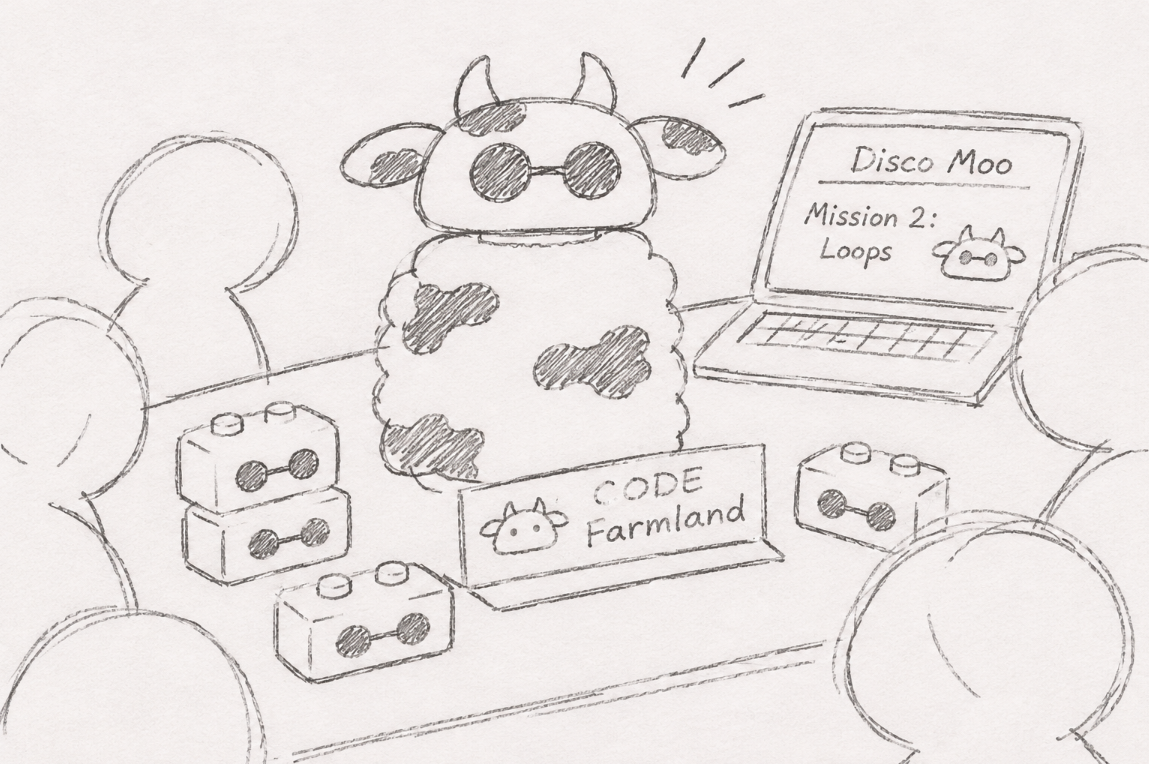
\includegraphics[width=\linewidth]{game_setting.png}}{\fbox{\parbox[c][1.25in][c]{0.9\linewidth}{\centering Placeholder: update game\_setting.png to depict Moo-d Lab, blocks, and mission screen.}}}
\caption{Proposed Moo-d Lab tabletop setting: cow-themed Reachy Mini, tangible coding blocks, a mission display, and collaborating students. The existing illustration can be updated to reflect the new emotion-themed game world.}
\label{fig:setting}
\end{figure}

\section{Robot Control Architecture}
\subsection{Architecture Design}
A hybrid, closed-loop finite-state machine (FSM) combines predefined motor routines with camera-driven decisions. States are READY, SCENARIO, ACTING, SCANNING, VALIDATING, EXECUTING, ACTOR\_RESPONSE, STORY\_OUTCOME, DEBUGGING, and CELEBRATING. The webpage presents a scenario and target programming constraint, cues the Actor, scans and validates the group program, executes it after the Actor's performance, and collects the Actor's selected reaction. The story engine then branches to a scripted consequence or retry. The screen provides story feedback; the robot provides embodied feedback. Scan failures and invalid syntax are handled separately from logical errors.

\subsection{Implementation Details}
Our Lab 4 camera interface detects paper ArUco markers and executes corresponding Reachy Mini movements. The proposed pipeline (1) detects marker IDs and ordering, (2) maps IDs to a constrained command vocabulary, (3) expands REPEAT instructions, (4) checks program validity, (5) executes safe robot movements, and (6) evaluates mission-specific rules and waits for the Actor's selected response before branching the story. The screen displays the recognized sequence and highlights the current command. The webpage mission engine stores target patterns for Missions 1--2; Mission 3 accepts any valid supported program, records the students' rationale, and uses a small authored branching story with Actor-selected reactions. Audio cues are prerecorded and triggered at defined points; they do not require a speech-generation pipeline. Remaining work includes reliable block scanning, loop interpretation, screen/robot synchronization, and feedback condition logic, plus a simple webpage interface for scripted actor prompts, reaction buttons, and story branches.

\subsection{Level of Autonomy}
After students request a scan, recognition, parsing, motion execution, rule-based evaluation, and screen/audio feedback are intended to run autonomously. Operators may initialize sessions, calibrate the camera, or recover from faults. Any Wizard-of-Oz assistance for transitions or audio will be recorded and reported separately.

\subsection{Architecture Diagram}
Figure~\ref{fig:architecture} shows how the physical program drives embodied action and narrative consequences. Student revision closes the loop.
\begin{figure}[H]
\centering
\fbox{\parbox[c]{0.92\linewidth}{\centering\small
\textbf{Webpage: Scenario + Actor Cue}\\
$\downarrow$\\
\textbf{Actor Performs; Team Builds / Scans}\\
$\downarrow$\\
\textbf{Camera + ArUco Detection and Ordering}\\
$\downarrow$\\
\textbf{Parser + Loop Expansion + Validation}\\
$\downarrow$\\
\textbf{FSM / Mission Rule Evaluator}\\
$\downarrow$\\
\textbf{Reachy Motor Actions + Audio Cues}\\
$\downarrow$\\
\textbf{Actor Selects Reaction; Webpage Branches}\\
$\downarrow$\\
\textbf{Group Discusses / Revises / Rescans}
}}
\caption{Physical--digital control loop linking narrative missions, tangible programming, embodied robot behavior, and student debugging.}
\label{fig:architecture}
\end{figure}

\section{Robot Design and Prototyping}
\subsection{Robot Design and Form}
We used \emph{sketching, storyboarding, 3D printing, and laser cutting} to develop the cow-themed Reachy Mini. Earlier concepts emphasized a disco-dancing cow; the revised Moo persona retains the playful costume and dance behavior but frames them as expressive responses to social situations. The character's visible eyes, head motion, and antennas support multiple possible expressions without requiring anthropomorphic claims about the robot's internal feelings. The storyboard now follows webpage scenario, Actor performance, group planning, block scanning, expressive robot response, Actor reaction, branching screen consequence, and revision.

\subsection{Fabrication and Materials}
A removable coat combines felt backing, white yarn, black yarn patches, hot glue, and adjustable retaining cords. Iteration replaced a poorly fitting flat wrap with a secure, removable fastening system designed not to obstruct cameras, ventilation, or movement. Interlocking coding blocks were 3D-printed, with socket tolerances of 14.00--14.03 mm tested for fit. A 5 mm wooden sign was laser-cut and engraved; its graphics can be relabeled for Moo-d Lab. ArUco labels on assembled blocks remain to be tested. Colored or icon-based block labels can reinforce the emotional theme without changing the underlying marker system.

\section{User Studies}
\subsection{Procedure}
At the K--12 demonstration, groups of four (or five) students will play for approximately 5--6 minutes, followed by 1--2 minutes of evaluation. An optional 8--10-minute extended session permits full role rotation and additional revisions. \textbf{(1) Setup:} verify camera recognition, webpage, connectivity, audio, and safe movement. \textbf{(2) Introduction:} introduce Moo and demonstrate a command block and the Actor's fictional role. \textbf{(3) Roles:} assign Actor, Director, Programmer, and Debugger; add Story Observer for groups of five. \textbf{(4) Gameplay:} webpage presents a scenario; Actor performs; teammates discuss, assemble, and scan a response; Reachy executes it. \textbf{(5) Story and feedback:} Actor selects a reaction, the webpage shows a predefined consequence, and students debug or revise as appropriate. Rotate the Actor at least once if feasible. \textbf{(6) Evaluation:} collect short programming items and an interpretation/rationale prompt. \textbf{(7) Reset:} restore blocks, webpage state, and robot pose. Research-team implementation and facilitation responsibilities will be coordinated across members; all members will contribute to technical integration and demonstration preparation.

\subsection{Game Testbed and Pre-study Setup}
The testbed includes a stable table, cow-costumed Reachy, approximately 8--12 blocks, a themed sign, a laptop running the story webpage, speakers or built-in audio output, scenario cards (or private actor prompts), and a marked scanning area. Pilot checks will cover lighting, marker visibility, command-order detection, loop parsing, motor limits, audio timing, and FSM reset, webpage story branching, and actor-response buttons. Scan failures will be logged separately from student programming errors. No ML model fine-tuning is needed for predefined ArUco recognition or rule-based evaluation.

\subsection{Evaluation: Study Design}
For \textbf{RQ1}, observers will document sequencing and repetition errors, scans, revisions, successful corrections, and participation across roles. For \textbf{RQ2}, the Actor will select whether Moo's response conveyed the intended social meaning, while the group briefly explains its movement choices. We will record agreement/disagreement, reasons, and whether students revise after the Actor's response; these measures reflect situated interpretation, not objective emotion accuracy. To reduce role confounding, we will note which student served as Actor and whether roles rotated.

For \textbf{H1}, groups will, if feasible, be assigned to \emph{A: specific encouraging debugging hints} or \emph{B: neutral mismatch notifications}. Both conditions use identical scenarios, blocks, visible recognized commands, and success rules. The primary outcome is the proportion of valid programming-error opportunities corrected on the next attempt; recognition failures are excluded. We will distinguish programming-error feedback from the Actor's social interpretation so the experimental manipulation is not conflated with story branching. Secondary outcomes include number of attempts, time to correction, mission completion, and qualitative coordination. With few groups and short sessions, findings will be descriptive and exploratory, even if the hypothesis is prespecified. We will document prior programming experience and any facilitator intervention.

\subsection{Evaluation: Measures}
Event-wide RoSAS~\cite{carpinella2017} and any available pre/post robot-perception questions will address warmth, competence, discomfort, and understanding of robots. Three brief computational-thinking items are:

\textbf{Q1 (sequencing):} What changes if LOOK RIGHT moves to the beginning of LOOK LEFT--NOD--LOOK RIGHT?

\textbf{Q2 (loops):} How can REPEAT 3 with NOD replace three NOD commands in Moo's happy dance?

\textbf{Q3 (debugging):} If Moo should LOOK LEFT--NOD--LOOK RIGHT but performs LOOK LEFT--LOOK RIGHT--NOD, what should be changed?

Each correct answer receives 1 point (total 0--3). Equivalent pre/post items will be used if time permits; otherwise scores are descriptive post-game evidence. A short optional prompt asks, ``Why did your team choose that movement for Moo's response?'' We will not infer durable learning or universal emotion recognition from a single brief session.

\section{Materials and Supplies}
\subsection{Materials for Game Components}
We will reuse one Reachy Mini, a removable cow costume, approximately 8--12 3D-printed blocks, a laser-cut sign, a computer, and printed ArUco labels. Existing audio hardware or laptop speakers will provide short prerecorded sound or music cues. The webpage displays scenario prompts, mission constraints, recognized code, Actor reaction choices, and authored story outcomes. The costume and physical blocks support character embodiment and tangible programming.

\subsection{Budget and Justification}
No new purchases are currently required; existing Lab 4 prototypes, equipment, and lab fabrication resources will be reused. Additional supplies, if needed, will require approval within the \$20 cap.
\begin{table}[H]
\centering
\caption{Requested supplies and budget.}
\label{tab:budget}
\begin{tabularx}{\linewidth}{@{}p{0.32\linewidth}Y@{}}
\hline
\textbf{Field} & \textbf{Requested item}\\
\hline
Supply & Existing blocks, costume, sign, computer/audio, and lab resources\\
Justification & Reuse Lab 4 prototypes and existing equipment\\
Additional quantity & 0\\
Unit price (\$) & 0.00\\
Line total (\$) & 0.00\\
Purchase URL & N/A; no purchase required\\
\hline
Total request (\$) & 0.00\\
\hline
\end{tabularx}
\end{table}

\begin{thebibliography}{00}
\bibitem{paper1} R. Sinha, H. Swanson, J. Clarke-Midura, J. F. Shumway, V. R. Lee, and S. Chandrasekharan, ``From Embodied Doing to Computational Thinking in Kindergarten: A Punctuated Motor Control Model,'' in \textit{Proc. ACM Symposium on Learning, Design and Technology}, 2023. doi: 10.1145/3594781.3594794.
\bibitem{paper2} C. De Jong, J. Peter, R. K\"uhne, and A. Barco, ``Children's Acceptance of a Domestic Social Robot: How It Evolves over Time,'' \textit{ACM Transactions on Human-Robot Interaction}, vol. 13, no. 2, art. 17, 2024. doi: 10.1145/3638066.
\bibitem{paper3} M. E. U. Ligthart, S. M. De Droog, M. Bossema, L. Elloumi, M. de Haas, M. H. J. Smakman, K. V. Hindriks, and S. Ben Allouch, ``Back to School---Sustaining Recurring Child-Robot Educational Interactions After a Long Break,'' in \textit{Proc. ACM/IEEE International Conference on Human-Robot Interaction}, 2024, pp. 433--442. doi: 10.1145/3610977.3635001.
\bibitem{paper4} A. Misirli and V. Komis, ``Computational thinking in early childhood education: The impact of programming a tangible robot on developing debugging knowledge,'' \textit{Early Childhood Research Quarterly}, vol. 65, pp. 139--158, 2023. doi: 10.1016/j.ecresq.2023.05.014.
\bibitem{carpinella2017} C.~M. Carpinella, A.~B. Wyman, M.~A. Perez, and S.~J. Stroessner, ``The Robotic Social Attributes Scale (RoSAS): Development and validation,'' in \textit{Proc. ACM/IEEE International Conference on Human-Robot Interaction}, 2017, pp. 254--262. doi: 10.1145/2909824.3020208.
\end{thebibliography}
\end{document}
